\section{Arquitectura}

En la figura \ref{fig:arquitectura} se muestra el diagrama de la arquitectura con la cual se trabajara para solventar la solución propuesta

%En la figura \ref{fig:arquitectura} se describirá la arquitectura propuesta para la solución de la problemática.

\begin{figure}[htb]
	\centering
	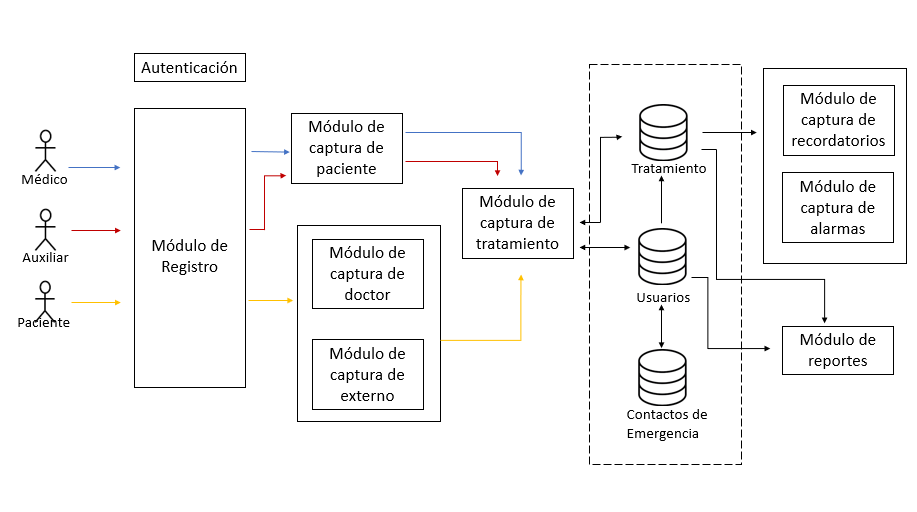
\includegraphics[width=0.8\textwidth]{images/cap2/Arquitectura}
	\caption{Arquitectura} \label{fig:arquitectura}
\end{figure}

Como podemos notar en la figura \ref{fig:arquitectura} se cuenta con cuatro actores que participaran en el sistema. Los cuales son :
\begin{itemize}
	\item Administrador
	\item Médico
	\item Paciente
	\item Externo
\end{itemize}

El actor \textbf{Administrador} sera el encargado de incluir los medicamentos que serán utilizados en los tratamientos.

El actor \textbf{Médico} dentro del sistema podrá agregar el tratamiento para el paciente.

El actor \textbf{Paciente} tendrá las siguientes acciones en el sistema :
\begin{itemize}
	\item Agregar el tratamiento medico.
	\item Modificar los recordatorios del tratamiento.
	\item Agregar contactos de emergencia.
	\item Consultar Reportes.
	\item Consultar Estadísticas.
	\item Consultar información de medicamentos.
	\item Creación de perfiles dependientes al \textbf{Paciente}.
\end{itemize}

El actor \textbf{Externo} nace de la necesidad de ayudar a los Pacientes que cuentan con poca o nula experiencia los dispositivos moviles o que por factores ajenas a la aplicación como son la de edad o alguna enfermedad les sea imposible utilizar la aplicación por si mismos. Es por eso que las acciones que tendrá en el sistema serán las mismas que las del paciente.

\section{Módulos}
La arquitectura contara con los siguientes módulos:
\begin{itemize}
	\item Módulo de Autenticación.
	\item Módulo captura de tratamientos.
	\item Módulo de recordatorios.
	\item Módulo de alarmas.
	\item Módulo de reportes.
	\item Módulo de estadísticas.
\end{itemize}

\textbf{Módulo Autenticación: } Este modulo es el encargado de verificar cual es tu perfil y darte acceso a los módulos correspondientes.

\textbf{Módulo captura de tratamientos: }Este módulo es el encargado de ingresar el tratamiento medico que expida el medico y asociar al perfil todos los detalles como lo son, los medicamentos, la dosis.

\textbf{Módulo de recordatorios: }Este módulo es el encargado de crear los recordatorios para el tratamiento medico asociado al perfil.

\textbf{Módulo de alarmas: }Este módulo se encargara de gestionar a tus contactos de emergencia y te permitirá editar convertir los recordatorios a alarmas de aquellos medicamentos que sean muy importantes.

\textbf{Módulo de reportes: }Este módulo generara un reporte en pdf que mostrara el tratamiento medico actual.

\textbf{Módulo de estadísticas:} Este módulo permitirá la visualización de información medica del paciente y de los medicamentos que toma.